% -*- coding: utf-8 -*-
% \protect{\ic(lambda (cnter~.~tmp) (set! tmp ...) (if ... (...~tmp) ...))}
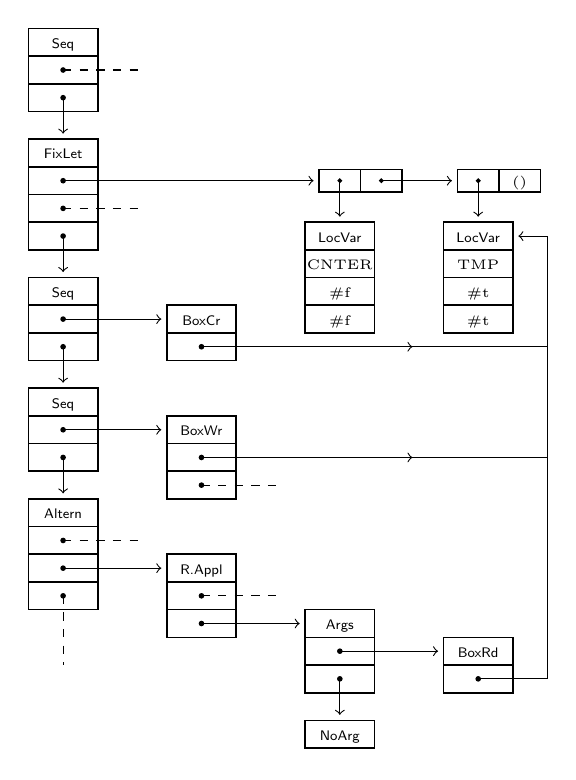
\begin{tikzpicture}
  \tikzstyle{every node}=[font=\tiny]

\def\NodeContent#1{\node [anchor = mid] at(1.25em, -0.5em) {#1};}
\def\NodeTitle#1{\NodeContent{\textsf{#1}}}
\def\NodePtr{\filldraw (1.25em, -0.5em) circle(0.8pt);}
\def\Box{\draw [semithick] (0, 0) rectangle (2.5em, -1.0em);}

\def\InList{%
  \begin{scope}[xshift = +0.5em, yshift = +1.5em]
    \draw [semithick] (0.0em, +0.4em) rectangle (3.0em, -0.4em)
                      (1.5em, +0.4em) -- (1.5em, -0.4em);
    \filldraw (0.75em, 0.0em) circle(0.65pt)
              (2.25em, 0.0em) circle(0.65pt);
  \end{scope}
}

\def\InListLast{%
  \begin{scope}[xshift = +0.5em, yshift = +1.5em]
    \draw [semithick] (0.0em, +0.4em) rectangle (3.0em, -0.4em)
                      (1.5em, +0.4em) -- (1.5em, -0.4em);
    \filldraw (0.75em, 0.0em) circle(0.65pt);
    \node [anchor = mid] at(2.25em, 0.0em) {\ic{()}};
  \end{scope}
}

\def\PullListLink{\draw [->] (-2.25em, 1.5em) -- (0.30em, 1.5em);}

\def\InBotList{%
  \begin{scope}[xshift = +0.5em, yshift = -1.5em]
    \draw [semithick] (0.0em, +0.4em) rectangle (3.0em, -0.4em)
                      (1.5em, +0.4em) -- (1.5em, -0.4em);
    \filldraw (0.75em, 0.0em) circle(0.65pt)
              (2.25em, 0.0em) circle(0.65pt);
  \end{scope}
}

\def\InBotListLast{%
  \begin{scope}[xshift = +0.5em, yshift = -1.5em]
    \draw [semithick] (0.0em, +0.4em) rectangle (3.0em, -0.4em)
                      (1.5em, +0.4em) -- (1.5em, -0.4em);
    \filldraw (0.75em, 0.0em) circle(0.65pt);
    \node [anchor = mid] at(2.25em, 0.0em) {\ic{()}};
  \end{scope}
}

\def\PullBotListLink{\draw [->] (-2.25em, -1.5em) -- (0.30em, -1.5em);}

\def\PullLinkUp{\draw    [->] ( 1.25em,  1.50em) -- ( 1.25em,  0.20em);}
\def\PullLinkLeft{\draw  [->] (-3.75em, -0.50em) -- (-0.20em, -0.50em);}
\def\PullLinkDown{\draw  [->] ( 1.25em, -1.50em) -- ( 1.25em, -0.20em);}
\def\PullLinkRight{\draw [->] ( 6.25em, -0.50em) -- ( 2.70em, -0.50em);}

\def\NoArgNode{%
  \begin{scope}[yshift = -0.0em]
    \Box
    \NodeTitle{NoArg}
  \end{scope}
}

\def\NoFreeNode{%
  \begin{scope}[yshift = -0.0em]
    \Box
    \NodeTitle{NoFree}
  \end{scope}
}

\def\PtrNodeU#1{%
  \begin{scope}[yshift = -0.0em]
    \Box
    \NodeTitle{#1}
  \end{scope}
  \begin{scope}[yshift = -1.0em]
    \Box
    \NodePtr
  \end{scope}
}

\def\ContentNode#1#2{
  \begin{scope}[yshift = -0.0em]
    \Box
    \NodeTitle{#1}
  \end{scope}
  \begin{scope}[yshift = -1.0em]
    \Box
    \NodeContent{#2}
  \end{scope}
}

\def\PtrNodeD#1{%
  \begin{scope}[yshift = -0.0em]
    \Box
    \NodeTitle{#1}
  \end{scope}
  \begin{scope}[yshift = -1.0em]
    \Box
    \NodePtr
  \end{scope}
  \begin{scope}[yshift = -2.0em]
    \Box
    \NodePtr
  \end{scope}
}

\def\ContentNodeD#1#2#3{
  \begin{scope}[yshift = -0.0em]
    \Box
    \NodeTitle{#1}
  \end{scope}
  \begin{scope}[yshift = -1.0em]
    \Box
    \NodeContent{#2}
  \end{scope}
  \begin{scope}[yshift = -2.0em]
    \Box
    \NodeContent{#3}
  \end{scope}
}

\def\PtrNodeDS#1{%
  \begin{scope}[yshift = -0.0em]
    \Box
    \NodeTitle{#1}
  \end{scope}
  \begin{scope}[yshift = -1.0em]
    \Box
    \begin{scope}[xshift = +0.35em]
      \NodePtr
    \end{scope}
  \end{scope}
  \begin{scope}[yshift = -2.0em]
    \Box
    \begin{scope}[xshift = -0.35em]
      \NodePtr
    \end{scope}
  \end{scope}
}

\def\PtrNodeT#1{
  \begin{scope}[yshift = -0.0em]
    \Box
    \NodeTitle{#1}
  \end{scope}
  \begin{scope}[yshift = -1.0em]
    \Box
    \NodePtr
  \end{scope}
  \begin{scope}[yshift = -2.0em]
    \Box
    \NodePtr
  \end{scope}
  \begin{scope}[yshift = -3.0em]
    \Box
    \NodePtr
  \end{scope}
}

\def\LocVarNode#1#2#3{
  \begin{scope}[yshift = -0.0em]
    \Box
    \NodeTitle{LocVar}
  \end{scope}
  \begin{scope}[yshift = -1.0em]
    \Box
    \NodeContent{#1}
  \end{scope}
  \begin{scope}[yshift = -2.0em]
    \Box
    \NodeContent{#2}
  \end{scope}
  \begin{scope}[yshift = -3.0em]
    \Box
    \NodeContent{#3}
  \end{scope}
}

\def\ClosureNode#1{
  \begin{scope}[yshift = -0.0em]
    \Box
    \NodeTitle{Closure}
  \end{scope}
  \begin{scope}[yshift = -1.0em]
    \Box
    \NodeContent{#1}
  \end{scope}
  \begin{scope}[yshift = -2.0em]
    \Box
    \NodePtr
  \end{scope}
  \begin{scope}[yshift = -3.0em]
    \Box
    \NodePtr
  \end{scope}
}

\def\FunDefNode#1{
  \begin{scope}[yshift = -0.0em]
    \Box
    \NodeTitle{FunDef}
  \end{scope}
  \begin{scope}[yshift = -1.0em]
    \Box
    \NodePtr
  \end{scope}
  \begin{scope}[yshift = -2.0em]
    \Box
    \NodePtr
  \end{scope}
  \begin{scope}[yshift = -3.0em]
    \Box
    \NodePtr
  \end{scope}
  \begin{scope}[yshift = -4.0em]
    \Box
    \NodeContent{#1}
  \end{scope}
}


\begin{scope}[xshift = 0.0em]
    \begin{scope}[yshift = -0.0em]
        \PtrNodeD{Seq}
    \begin{scope}[yshift = -4.0em]
        \PullLinkUp
        \PtrNodeT{FixLet}
    \begin{scope}[yshift = -5.0em]
        \PullLinkUp
        \PtrNodeD{Seq}
    \begin{scope}[yshift = -4.0em]
        \PullLinkUp
        \PtrNodeD{Seq}
    \begin{scope}[yshift = -4.0em]
        \PullLinkUp
        \PtrNodeT{Altern}
    \end{scope}\end{scope}\end{scope}
    \end{scope}\end{scope}
\end{scope}

% Seq ->
\draw [dashed] (1.25em,  -1.50em) -- (4.00em,  -1.50em);

% FixLet -> LocVarList
\draw [->] (1.25em, -5.50em) -- (10.30em, -5.50em);

% FixLet ->
\draw [dashed] (1.25em,  -6.50em) -- (4.00em,  -6.50em);

% Altern -> 
\draw [dashed] (1.25em, -18.50em) -- (4.00em, -18.50em);
\draw [dashed] (1.25em, -20.50em) -- (1.25em, -23.00em);

\begin{scope}[xshift = 5.0em]
    \begin{scope}[yshift = -10.0em]
        \PullLinkLeft
        \PtrNodeU{BoxCr}
    \begin{scope}[yshift = -4.0em]
        \PullLinkLeft
        \PtrNodeD{BoxWr}
    \begin{scope}[yshift = -5.0em]
        \PullLinkLeft
        \PtrNodeD{R.Appl}
    \end{scope}\end{scope}\end{scope}
\end{scope}

% BoxCr -> TMP
\draw [->] ( 6.25em, -11.50em) -- (13.875em, -11.50em);
\draw      (13.50em, -11.50em) -- (18.750em, -11.50em);

% BoxWr -> TMP
\draw [->] ( 6.25em, -15.50em) -- (13.875em, -15.50em);
\draw      (13.50em, -15.50em) -- (18.750em, -15.50em);

% BoxWr ->
\draw [dashed] (6.25em, -16.50em) -- (9.00em, -16.50em);

% R.Appl ->
\draw [dashed] (6.25em, -20.50em) -- (9.00em, -20.50em);

\begin{scope}[xshift = 10.0em]
    \begin{scope}[yshift =  -7.0em]
        \InList
        \PullLinkUp
        \LocVarNode{\ic{CNTER}}{\ic{\#f}}{\ic{\#f}}
    \begin{scope}[yshift = -14.0em]
        \PullLinkLeft
        \PtrNodeD{Args}
    \begin{scope}[yshift =  -4.0em]
        \PullLinkUp
        \NoArgNode
    \end{scope}\end{scope}\end{scope}
\end{scope}

\begin{scope}[xshift = 15.0em]
    \begin{scope}[yshift =  -7.0em]
        \InListLast
        \PullLinkUp
        \PullListLink
        \LocVarNode{\ic{TMP}}{\ic{\#t}}{\ic{\#t}}
    \begin{scope}[yshift = -15.0em]
        \PullLinkLeft
        \PtrNodeU{BoxRd}
    \end{scope}\end{scope}
\end{scope}

% BoxRd -> TMP
\draw [->] (16.25em, -23.50em) -- (18.75em, -23.50em) --
           (18.75em,  -7.50em) -- (17.70em,  -7.50em);

\end{tikzpicture}
